\documentclass{beamer}

\usetheme{metropolis}

\usepackage{color}
\usepackage{soul}
\usepackage{tikz}
\usepackage{xcolor}

\usetikzlibrary{calc}

\date{13.02.23}
\title{What is a JSON file}
\author{Esten H. Leonardsen}

\begin{document}
	\begin{frame}
	 	\maketitle
	\end{frame}

	\begin{frame}
		\centering
		\huge{JavaScript Object Notation}
	\end{frame}

	\begin{frame}
		\begin{tikzpicture}
			\node[] (car) at (0, 0) {
				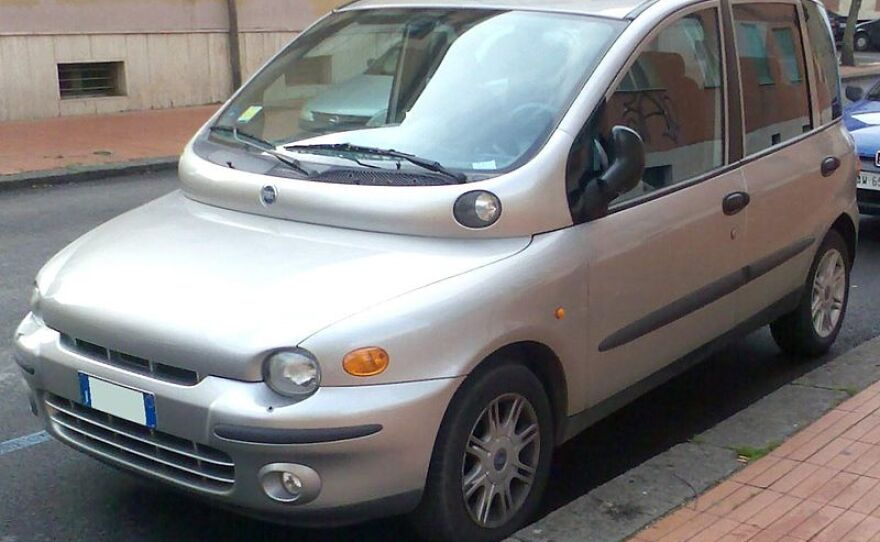
\includegraphics[width=2cm]{data/car.jpeg}
			};

			\node[anchor=north west] at ($ (car.east) + (2.6, 1) $) {
				\tiny
				\begin{tabular}{|c|c|c|c|c|}
					\hline
					\textbf{Manufacturer}&\textbf{Model}&\textbf{Year}&\textbf{Color}&\textbf{HP}\\
					\hline
					Fiat&Multipla&1998&Gray&120\\
					\hline
				\end{tabular}
			};
			\node[] at (-1, 1) {};
			\node[] at (10, -2.2) {};
		\end{tikzpicture}
	\end{frame}

	\begin{frame}
		\begin{tikzpicture}
			\node[] (car) at (0, 0) {
				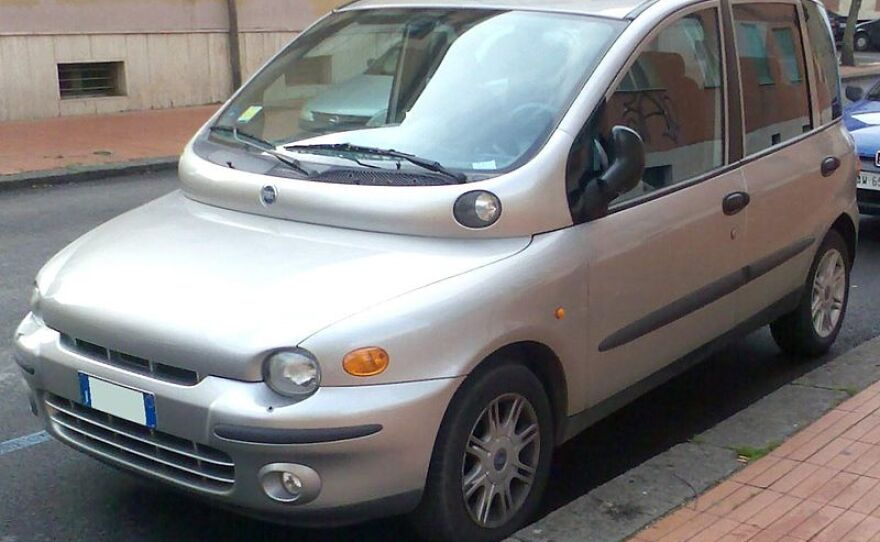
\includegraphics[width=2cm]{data/car.jpeg}
			};
			\node[anchor=south west] at (car.south east) {
				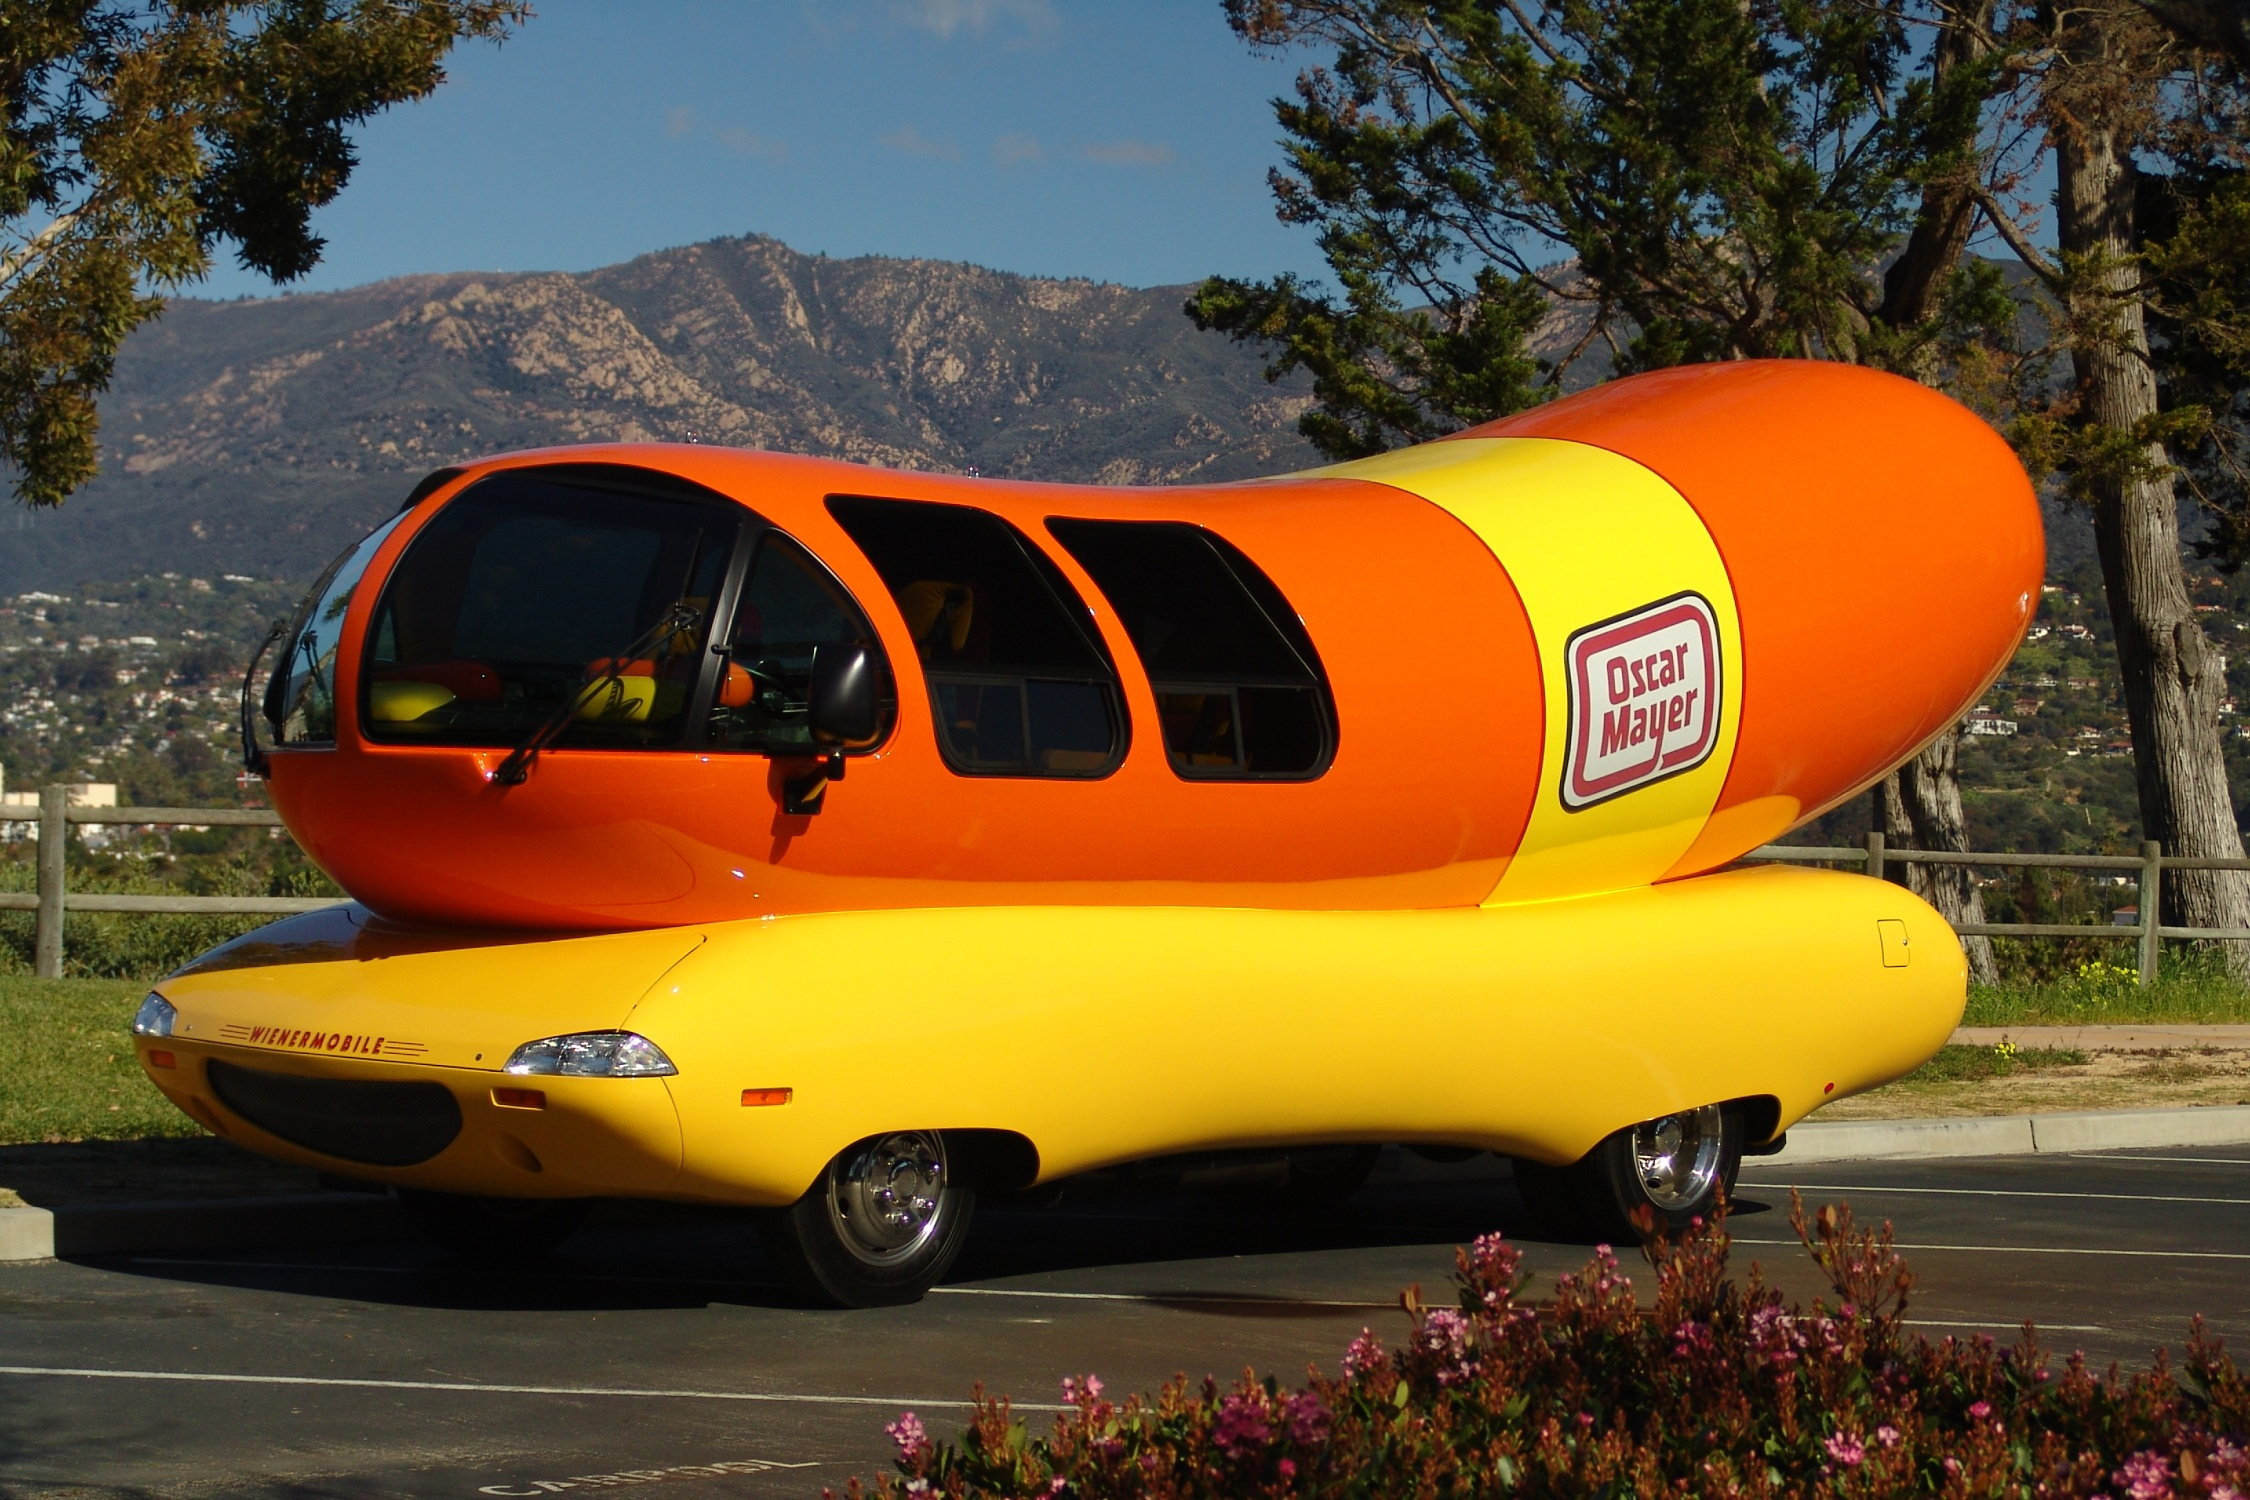
\includegraphics[width=2cm]{data/hotdogcar.jpg}
			};
			\node[anchor=north east] at (car.south east) {
				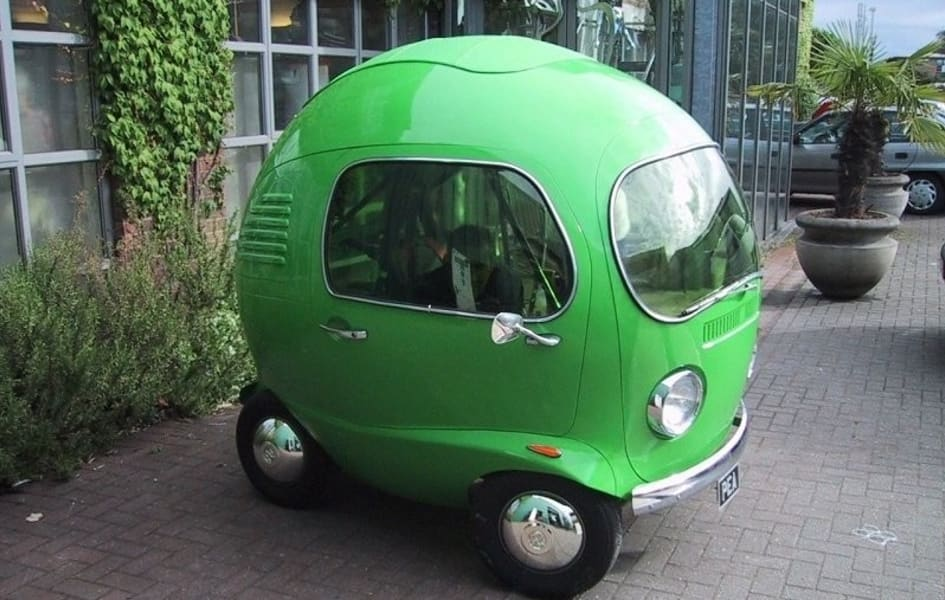
\includegraphics[width=2cm]{data/greencar.jpeg}
			};
			\node[anchor=north west] at (car.south east) {
				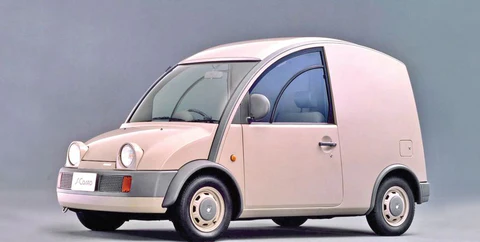
\includegraphics[width=2cm]{data/pinkcar.png}
			};

			\node[anchor=north west] at ($ (car.east) + (2.6, 1) $) {
				\tiny
				\begin{tabular}{|c|c|c|c|c|}
					\hline
					\textbf{Manufacturer}&\textbf{Model}&\textbf{Year}&\textbf{Color}&\textbf{HP}\\
					\hline
					Fiat&Multipla&1998&Gray&120\\
					\hline
					Oscar-Mayer&Wienercar&2005&Yellow&150\\
					\hline
					Asylum&Pea Car&1995&Green&850\\
					\hline
					Nissan&X-Cargo&1972&Pink&75\\
					\hline
				\end{tabular}
			};
			\node[] at (-1, 1) {};
			\node[] at (10, -2.2) {};
		\end{tikzpicture}
	\end{frame}

	\begin{frame}
		\centering
		\vfill
		\begin{tikzpicture}
			\node[] (car) at (0, 0) {
				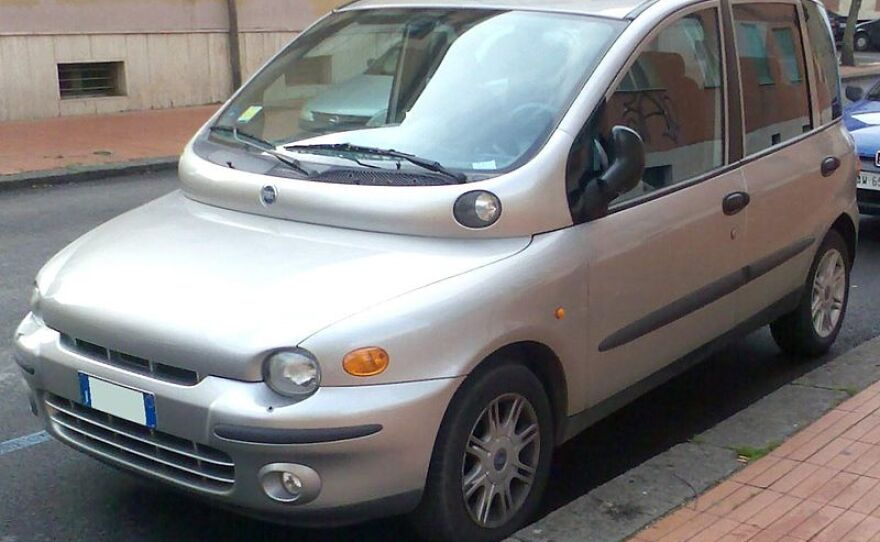
\includegraphics[width=3cm]{data/car.jpeg}
			};

			\node[anchor=north west, align=left,font=\scriptsize] at ($ (car.north east) + (1, 2.65) $) {
				\{\\
				\quad manufacturer: "Fiat",\\
				\quad model: "Multipla",\\
				\quad year: 1998,\\
				\quad color: "gray",\\
				\quad horse\_power: 120\\
				\}
			};
			\node[] at (-1.4, 3.75) {};
			\node[] at (8.5, -3.75) {};
		\end{tikzpicture}
		\vfill
	\end{frame}

	\begin{frame}
		\centering
		\vfill
		\begin{tikzpicture}
			\node[] (car) at (0, 0) {
				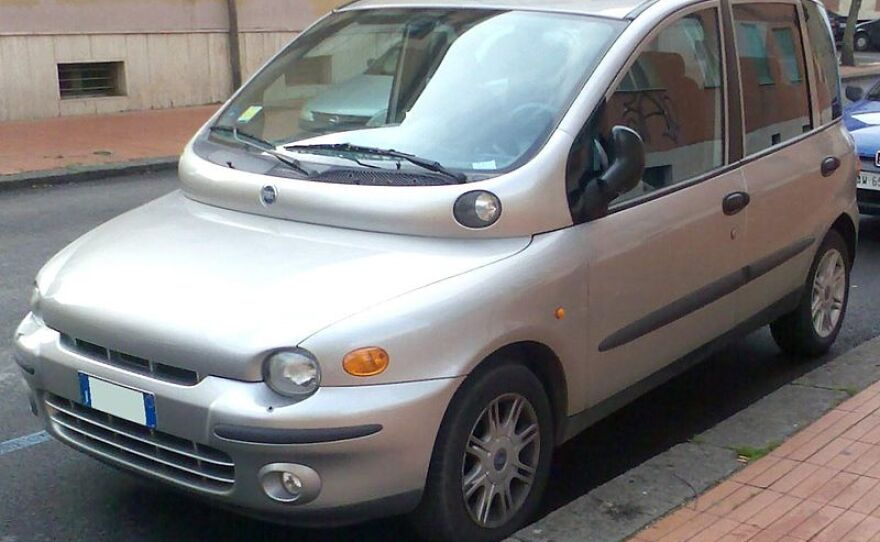
\includegraphics[width=3cm]{data/car.jpeg}
			};

			\node[anchor=north west, align=left,font=\scriptsize] at ($ (car.north east) + (1, 2.65) $) {
				\{\\
				\quad manufacturer: "Fiat",\\
				\quad model: "Multipla",\\
				\quad year: 1998,\\
				\quad color: "gray",\\
				\quad horse\_power: 120,\\
				\quad tire\_manufacturer: "Goodyear",\\
				\quad tire\_pressure: 35,\\
				\quad tire\_depth: 8\\
				\}
			};
			\node[] at (-1.4, 3.75) {};
			\node[] at (8.5, -3.75) {};
		\end{tikzpicture}
		\vfill
	\end{frame}

	\begin{frame}
		\centering
		\vfill
		\begin{tikzpicture}
			\node[] (car) at (0, 0) {
				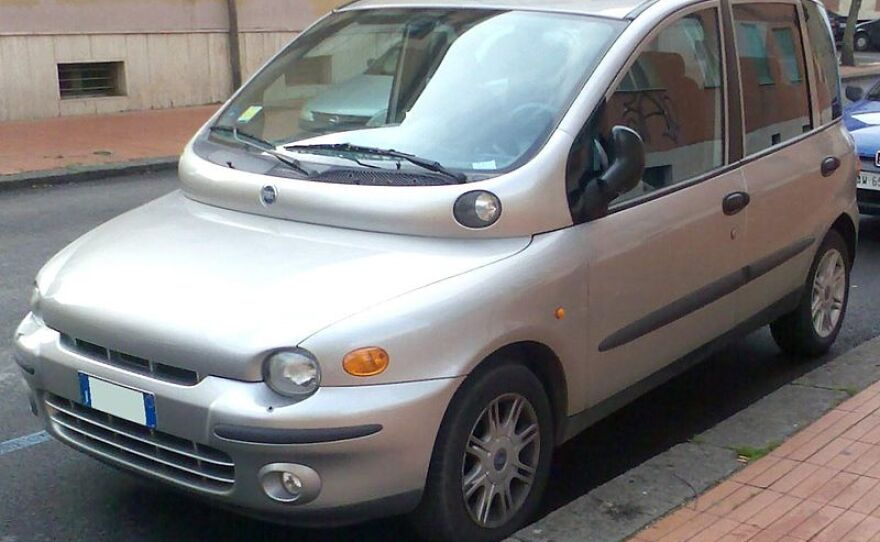
\includegraphics[width=3cm]{data/car.jpeg}
			};

			\node[anchor=north west, align=left,font=\scriptsize] at ($ (car.north east) + (1, 2.65) $) {
				\{\\
				\quad manufacturer: "Fiat",\\
				\quad model: "Multipla",\\
				\quad year: 1998,\\
				\quad color: "gray",\\
				\quad horse\_power: 120,\\
				\quad left\_front\_tire\_manufacturer: "Goodyear",\\
				\quad left\_front\_tire\_pressure: 35,\\
				\quad left\_front\_tire\_depth: 8,\\
				\quad left\_rear\_tire\_manufacturer: "Goodyear",\\
				\quad left\_rear\_tire\_pressure: 33,\\
				\quad left\_rear\_tire\_depth: 7,\\
				\quad right\_front\_tire\_manufacturer: "Goodyear",\\
				\quad right\_front\_tire\_pressure: 32,\\
				\quad right\_front\_tire\_depth: 7,\\
				\quad right\_rear\_tire\_manufacturer: "Continental",\\
				\quad right\_rear\_tire\_pressure: 35,\\
				\quad right\_rear\_tire\_depth: 6\\
				\}
			};
			\node[] at (-1.4, 3.75) {};
			\node[] at (8.5, -3.75) {};
		\end{tikzpicture}
		\vfill
	\end{frame}

	\begin{frame}
		\centering
		\vfill
		\begin{tikzpicture}
			\node[] (car) at (0, 0) {
				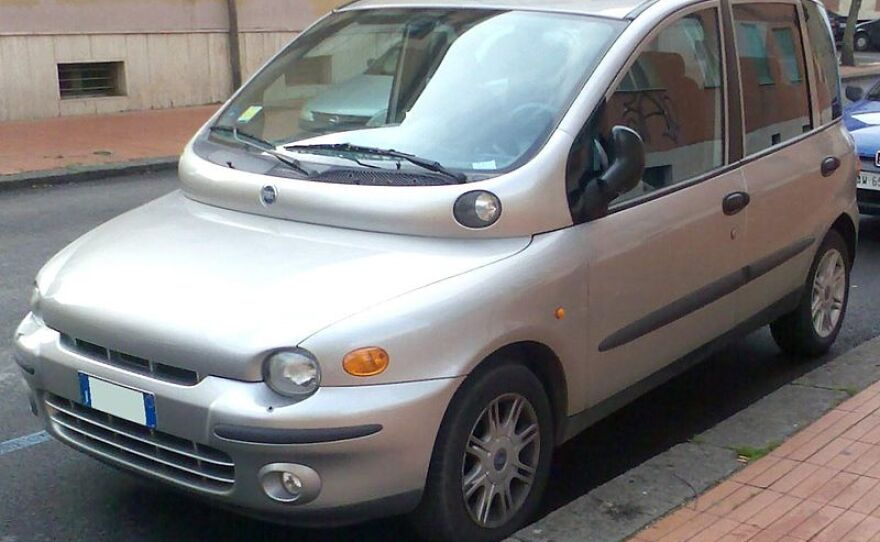
\includegraphics[width=3cm]{data/car.jpeg}
			};

			\node[anchor=north west, align=left,font=\scriptsize] at ($ (car.north east) + (1, 2.65) $) {
				\{\\
				\quad manufacturer: "Fiat",\\
				\quad model: "Multipla",\\
				\quad year: 1998,\\
				\quad color: "gray",\\
				\quad horse\_power: 120,\\
				\quad left\_front\_tire: \{\\
				\quad\quad manufacturer: "Goodyear",\\
				\quad\quad pressure: 35,\\
				\quad\quad depth: 8\\
				\quad \},\\
				\quad left\_rear\_tire: \{\\
				\quad\quad manufacturer: "Goodyear",\\
				\quad\quad pressure: 33,\\
				\quad\quad depth: 7\\
				\quad \},\\
				\quad \ldots\\
				\}
			};
			\node[] at (-1.4, 3.75) {};
			\node[] at (8.5, -3.75) {};
		\end{tikzpicture}
		\vfill
	\end{frame}

	\begin{frame}
		\centering
		\vfill
		\begin{tikzpicture}
			\node[] (car) at (0, 0) {
				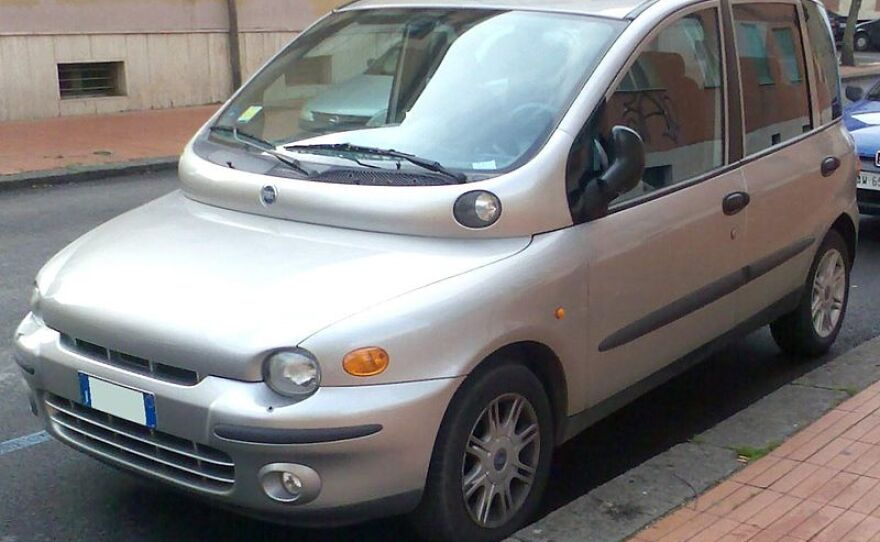
\includegraphics[width=3cm]{data/car.jpeg}
			};

			\node[anchor=north west, align=left,font=\scriptsize] at ($ (car.north east) + (1, 2.65) $) {
				\{\\
				\quad manufacturer: "Fiat",\\
				\quad model: "Multipla",\\
				\quad year: 1998,\\
				\quad color: "gray",\\
				\quad horse\_power: 120,\\
				\quad left\_front\_tire: \{\\
				\quad\quad manufacturer: "Goodyear",\\
				\quad\quad pressure: 35,\\
				\quad\quad depth: 8\\
				\quad\quad valve: \{\\
				\quad\quad\quad manufacturer: "Schrader",\\
				\quad\quad\quad diameter: 0.2\\
				\quad\quad \}\\
				\quad \},\\
				\quad \ldots\\
				\}
			};
			\node[] at (-1.4, 3.75) {};
			\node[] at (8.5, -3.75) {};
		\end{tikzpicture}
		\vfill
	\end{frame}

	\begin{frame}
		\centering
		\vfill
		\begin{tikzpicture}
			\node[] (car) at (0, 0) {
				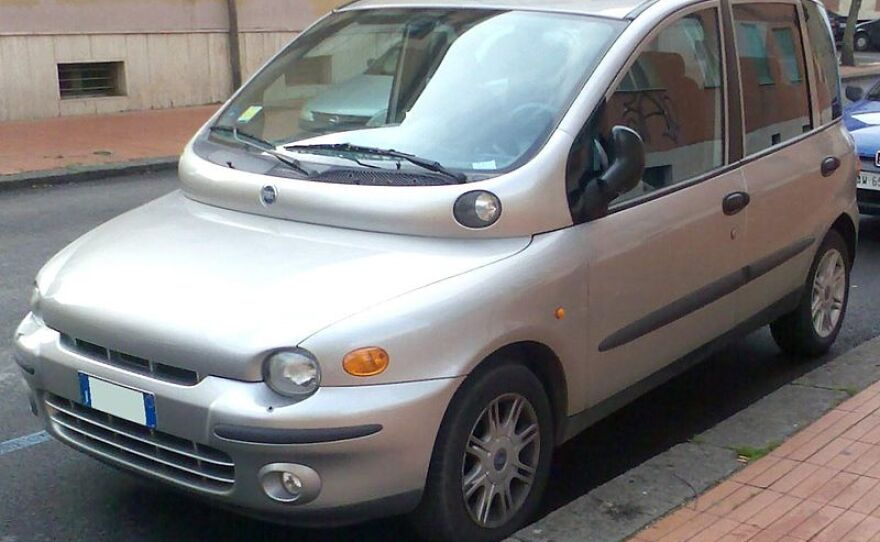
\includegraphics[width=3cm]{data/car.jpeg}
			};

			\node[anchor=north west, align=left,font=\scriptsize] at ($ (car.north east) + (1, 2.65) $) {
				\{\\
				\quad "manufacturer": "Fiat",\\
				\quad "model": "Multipla",\\
				\quad "year": 1998,\\
				\quad "color": "gray",\\
				\quad "horse\_power": 120,\\
				\quad "left\_front\_tire": \{\\
				\quad\quad "manufacturer": "Goodyear",\\
				\quad\quad "pressure": 35,\\
				\quad\quad "depth": 8\\
				\quad\quad "valve": \{\\
				\quad\quad\quad "manufacturer": "Schrader",\\
				\quad\quad\quad "diameter": 0.2\\
				\quad\quad \}\\
				\quad \},\\
				\quad \ldots\\
				\}
			};
			\node[] at (-1.4, 3.75) {};
			\node[] at (8.5, -3.75) {};
		\end{tikzpicture}
		\vfill
	\end{frame}

	\begin{frame}
		\centering
		\vfill
		\begin{tikzpicture}
			\node[] (car) at (0, 0) {
				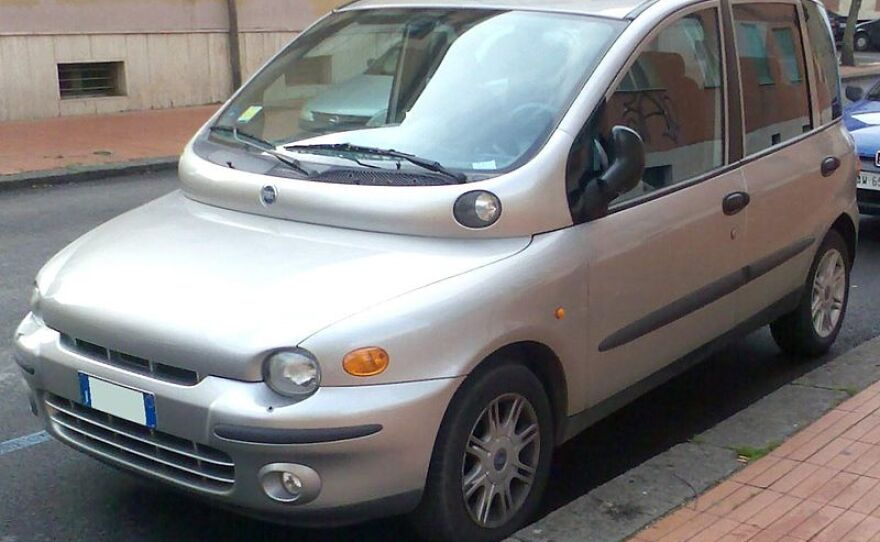
\includegraphics[width=3cm]{data/car.jpeg}
			};

			\node[anchor=north west, align=left,font=\scriptsize] at ($ (car.north east) + (1, 2.65) $) {
				\{\\
				\quad \textcolor{red}{"manufacturer"}: \textcolor{green}{"Fiat"},\\
				\quad "model": "Multipla",\\
				\quad "year": 1998,\\
				\quad "color": "gray",\\
				\quad "horse\_power": 120,\\
				\quad "left\_front\_tire": \{\\
				\quad\quad "manufacturer": "Goodyear",\\
				\quad\quad "pressure": 35,\\
				\quad\quad "depth": 8\\
				\quad\quad "valve": \{\\
				\quad\quad\quad "manufacturer": "Schrader",\\
				\quad\quad\quad "diameter": 0.2\\
				\quad\quad \}\\
				\quad \},\\
				\quad \ldots\\
				\}
			};
			\node[] at (-1.4, 3.75) {};
			\node[] at (8.5, -3.75) {};

			\node[] at (3.5, -3.2) {\scriptsize{\textcolor{red}{Key: Text string enclosed by double quotes}}};
			\node[] at (3.5, -3.55) {\scriptsize{\textcolor{green}{Value: Text string, integer, floating-point number, JSON-object, list of JSON-objects}}};
		\end{tikzpicture}
		\vfill
	\end{frame}
\end{document}
